\section{内視鏡画像からの簡易カルテ自動生成システム}

提案手法をデータセットの作成、モデルの作成、モデルの学習、評価指標から説明する。
すべての実装コードは筆者のgithubのレポジトリ (https://github.com/shinn1r0\\/endoscopic\_images2karte)にある。
実装には主にPythonを用い、深層学習フレームワークにはPytorchを使用した。
またプライバシー情報のためデータセット作成の元となる内視鏡画像と簡易カルテのデータ、それらから生成したデータセットは含まれていない。
\subsection{データセットの作成}
本論文では画像を個別にマルチラベルと関連付けで学習する手法と各患者ごとの全ての画像をまとめてマルチラベルと関連付けで学習する手法の二つの手法で実験を行ったため、データセットも二つ用意した。
簡易カルテからのマルチラベル生成と各画像における処理は共通であるが、その後の処理はそれぞれの手法で異なる。
\subsubsection{簡易カルテからのマルチラベル生成}

\begin{figure}[tb]
    \begin{center}
        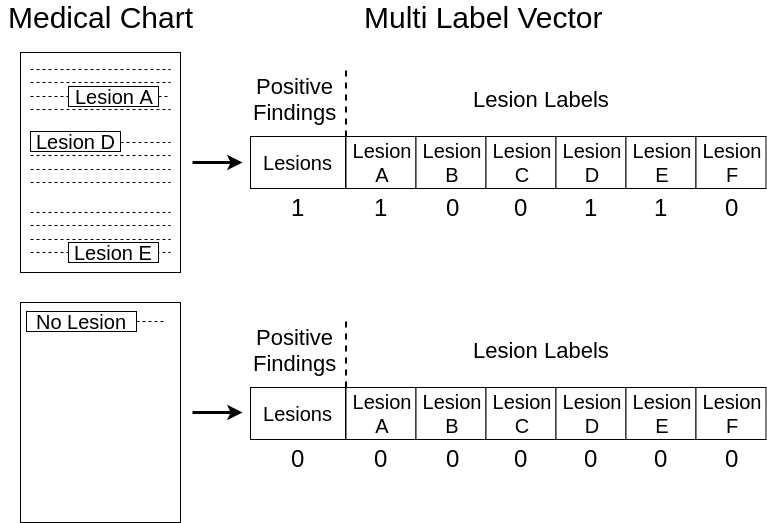
\includegraphics[width=75mm]{./fig/ieice1.png}
        \caption{Dataset Creation}
        \label{fig:multilabel}
    \end{center}
\end{figure}

簡易カルテからのマルチラベル生成 (図\ref{fig:multilabel})は以下の手順で行った。

\begin{enumerate}
    \item すべて異常なしの患者を抽出
    \item 簡易カルテ内の質的診断を言語処理
    \item 処理後の内容を全ての患者でまとめてカテゴリー化
    \item 頻出病名カテゴリー選択
    \item 各患者ごとにマルチラベル生成
    \item マルチラベルのone-hotベクトル化
\end{enumerate}

詳細を述べる。
 (1)では簡易カルテ内の全ての行で異常なしとなっている患者を抜き出し、 (2)から (4)の処理には通していない。
 (2)では簡易カルテ内の質的診断の項目のみを取り出し、言語処理を行った。
この言語処理では文書であったり単語や数値の羅列であったりする質的診断をまず単語の系列データへと変換した。
次にこれらを形態素解析や事前に用意した病名リストを用いた検索などを通して病名を表す単語とそれらに付随する情報を示す単語を抽出した。
その際に複雑な付随情報を持つような病名は固有の処理を加えている。
これにより簡易カルテの質的診断の項目では、各行が、先頭に病名単語があり、その後に付加情報単語が続く形式になった。 
(3)では (2)の処理後の内容を全ての患者を通して集計し、同じ単語を同じラベル付けをして辞書に格納した。 
(4)では辞書内で出現回数を計測し、指定した回数以上のラベルを頻出病名ラベルとして決定した。
本研究ではすべて頻出病名を15個に設定した。
 (5) (6)では各患者ごとにone-hot化したマルチラベルを生成した。
マルチラベルは1番目のラベルには異常が一つでもある患者は1を、それ以外の患者は0が格納されている。これには (1)で抽出した情報を用いた。
マルチラベルの2番目以降のラベルには頻出病名ラベルがある。 
(2)から (4)で作成した情報を元に、各患者の質的診断の項目に頻出病名が存在する場合は1を、存在しない場合は0が格納されている。
\subsubsection{各画像における処理}
すべての画像は$256 \times 256$ピクセルにサイズ変更した。
その後画像のRGBチャンネルそれぞれを正規化した。
正規化のパラメータはRが平均0.485、標準偏差0.229、Gが平均0.456、標準偏差0.224、Bが平均0.406、標準偏差0.225に設定した。
これらの値はすべて深層学習フレームワークのPytorchで推奨されている値を用いた。
\subsubsection{データセット分割}
2つの手法に合わせてデータセットを2つ用意した。
それぞれのデータセットは訓練データ、検証データ、テストデータに分割した。
\begin{itemize}
    \item 画像を個別に入力する手法\\
この手法では、学習に用いる訓練データと検証データは画像を全患者に渡ってランダムにし、それぞれをマルチラベルと関連付けした。
それに対して、テストでは患者単位での予測になるために、テストデータは患者単位で検査順に並んだ画像を系列データとしてマルチラベルと関連付けした。
    \item 画像を患者ごとにまとめて入力する手法\\
この手法では、学習とテストに用いる全てのデータを患者単位でまとめた。
データは検査順に並べた画像を時間軸で連結させ、三次元データとし、それぞれマルチラベルと関連付けした。
\end{itemize}

\subsection{モデルの作成}
2つの手法に合わせてモデルも2つ用意した。
どちらのモデルでも残差構造を持っていて、表現力の大きい多層のCNNを用いている。
モデルの選択はPytorchで安定的に良い性能があるとされていて、用いられることが多いものを参考にした。
\begin{itemize}
    \item 画像を個別に入力する手法\\
この手法では残差構造 (Residential Connect)を持つCNN\cite{CNN}で最も一般的なResNet\cite{ResNet}を発展させたDenseNet\cite{DenseNet}を用いた。
残差構造では、従来のネットワークでは同じ深さの層では同じ大きさの特徴しか抽出できなかったのに対して、ショートカットを用いることで同じ深さの層でも異なる大きさの特徴を抽出できるようになっている。
ResNetはネットワークの主要部分で畳み込みを行って、ショートカット部分でその畳み込みを飛ばす構造をしている。
DenseNetでは主要部分では畳み込みを行わず、分岐した部分に設置したDense Blockによって畳み込みを行い、その出力が主要部分で合流する構造をしている。
これによりResNetより少ないパラメータ数で効率良く特徴抽出ができることが確認されている。
    \item 画像を患者ごとにまとめて入力する手法\\
この手法では画像を連結した三次元データを入力するため、CNNを三次元に拡張した3D-CNNを用いた。
3D-CNNの中でも現在最も良い性能を持っている3D-ResNet\cite{3D_ResNet}を選択した。
\end{itemize}

\subsubsection{DenseNetのチューニング}

\begin{figure}[tb]
    \begin{center}
        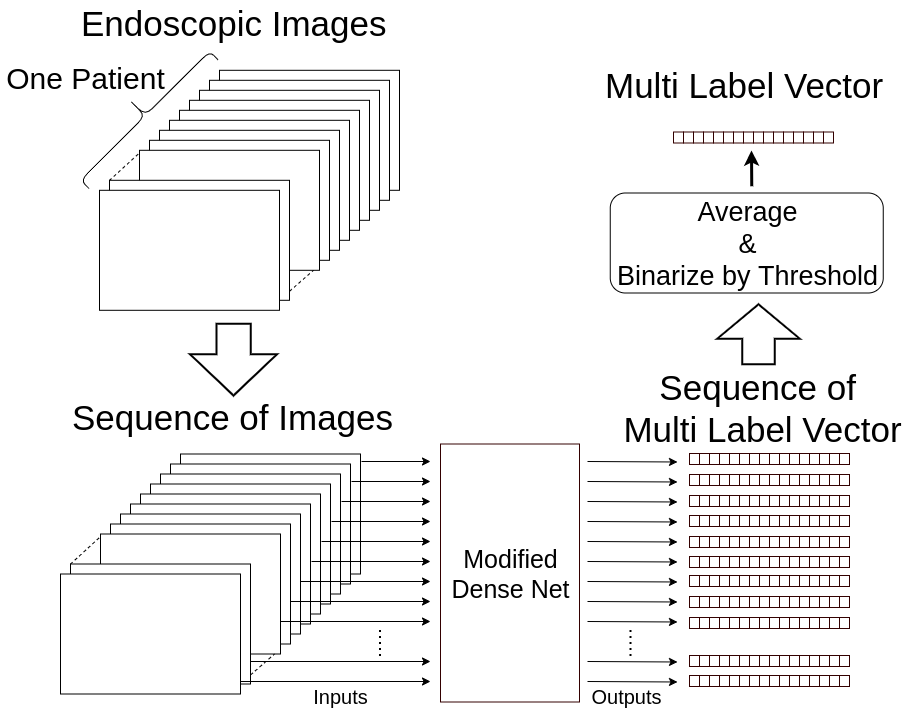
\includegraphics[width=75mm]{./fig/ieice2.png}
        \caption{DenseNet}
        \label{fig:densenet}
    \end{center}
\end{figure}

本研究に合わせてDenseNet (図\ref{fig:densenet})のチューニングをし、複数のモデルを用意した。
全てのモデルにおいて共通していることは、特徴抽出部分をそのまま用いていることと、分類器部分の最終層のニューロン数をマルチラベルのクラス数と合わせていることである。
これに加えて分類器部分を、通常の一層の全結合層のみの構造から、複数の全結合層とバッチ正規化とドロップアウトをからなる構造に変更したものも用意した。
これはマルチラベル予測においては、抽出した特徴の組み合わせが1つのラベルの予測よりも複雑になるために、分類器においても深層の構造を用いて対応するためである。
また今回の実験ではより複雑な特徴にも対応するために、層の数の異なる2つのDenseNetで学習した。
それぞれDenseNet121\cite{DenseNet}とDenseNet161\cite{DenseNet}というモデルを用いた。
このため合わせて4パターンで実験を行った。
\subsubsection{3D-ResNetのチューニング}

\begin{figure}[tb]
    \begin{center}
        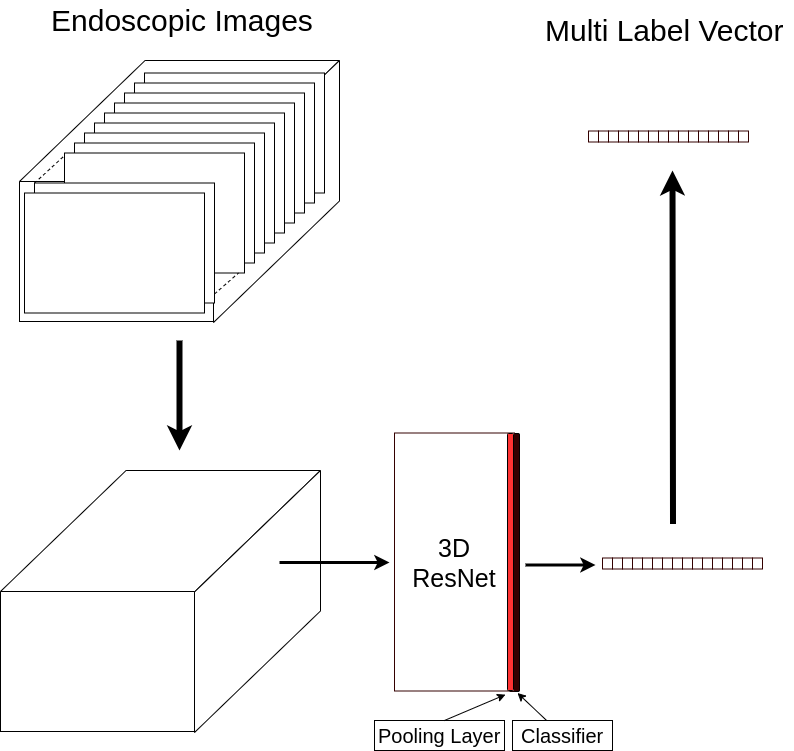
\includegraphics[width=75mm]{./fig/ieice3.png}
        \caption{3D-ResNet}
        \label{fig:3d_resnet}
    \end{center}
\end{figure}

本研究に合わせて3D-ResNet (図\ref{fig:3d_resnet})のチューニングをし、複数のモデルを用意した。
特徴抽出部分の最終層において、通常では平均プーリングをして特徴を合算している。
その際に特徴が損失する恐れがあったため、これを最大プーリングに置き換えたものも用意した。
また分類器部分でもDenseNetのときと同じように、一層の全結合層のみのものと、複数の全結合層とバッチ正規化とドロップアウトをからなる構造に変更したものを用意した。
このため合わせて4パターンで実験を行った。
